
%(BEGIN_QUESTION)
% Copyright 2006, Tony R. Kuphaldt, released under the Creative Commons Attribution License (v 1.0)
% This means you may do almost anything with this work of mine, so long as you give me proper credit

Anta at vi fyller væske jevnt i det venstre vertikale røret til nivået når et merke fire tommer over bunnen.  Gitt diameterne på de andre rørene: hvor høyt vil væskenivået stabilisere seg i hvert rør når alle søyler er i likevekt (ingen væske {\it strømmer} noe sted i systemet)?

$$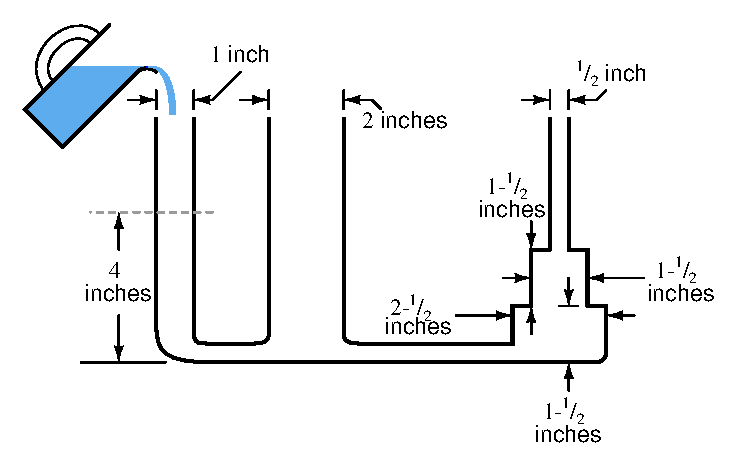
\includegraphics[width=15.5cm]{i00236x01.eps}$$

Vurder nå det samme settet med vertikale rør (samme diametre, samme trinnhøyder) koblet sammen i bunnen med et {\it skrått} rør.  Hvis vi fyller væske i det venstre vertikale røret til nivået når et merke to tommer over bunnen: hvor høyt vil væskenivået stabilisere seg i hver søyle når alle søyler er i likevekt?

$$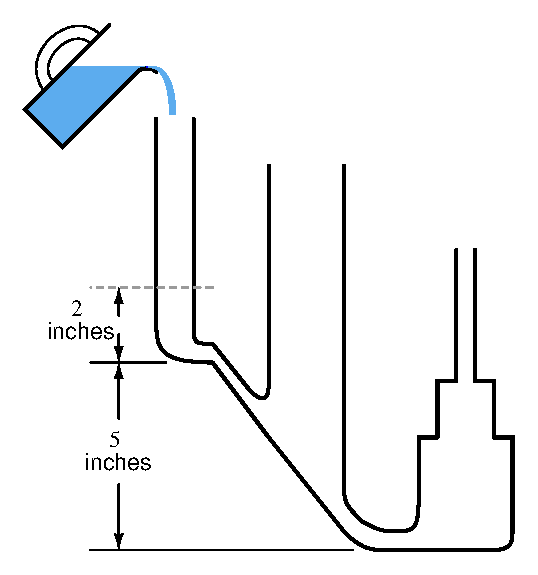
\includegraphics[width=9cm]{i00236x03.eps}$$

\underbar{file i00236}
%(END_QUESTION)





%(BEGIN_ANSWER)

$$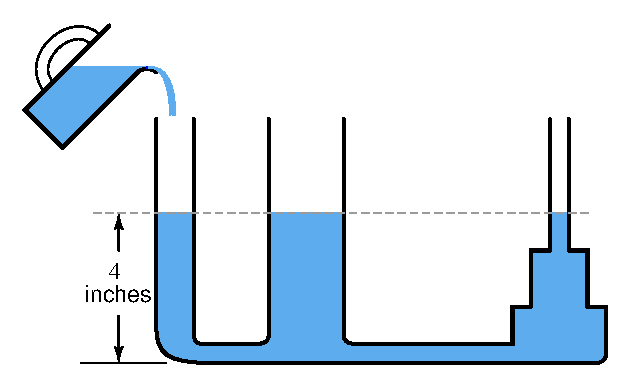
\includegraphics[width=15.5cm]{i00236x02.eps}$$

$$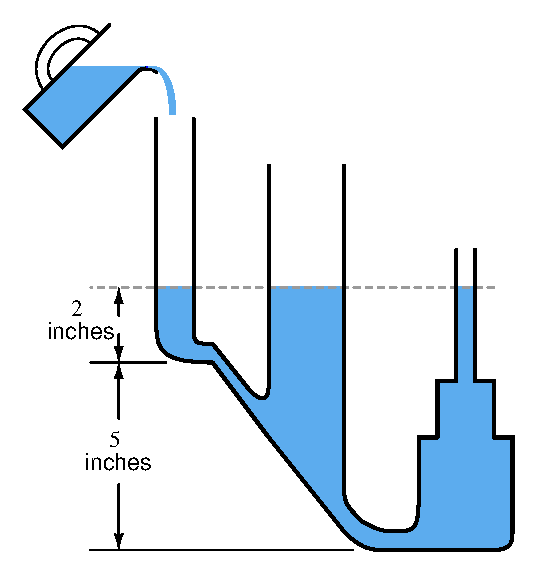
\includegraphics[width=15.5cm]{i00236x04.eps}$$

%(END_ANSWER)





%(BEGIN_NOTES)

I begge tilfeller vil væskenivået være helt likt når det måles relativt til bakkenivå.  I likevektstilstand er alle krefter i systemet balansert.  Det betyr at hydrostatisk trykk i hver søyle er det samme, altså samme væskehøyde i hver søyle.

Diameter og form på de enkelte søylene spiller ingen rolle.  Alle oppgitte mål for diameter og trinnhøyde i høyre søyle er irrelevante.  Den enkle avhengigheten hydrostatisk trykk har av søylehøyde, væsketetthet og tyngdeakselerasjon gjør statiske væskesøyler svært enkle å analysere.

%INDEX% Physics, static fluids: equal height of bottom-connected liquid columns

%(END_NOTES)
